\documentclass[tikz,border=3pt]{standalone}
\usepackage[utf8]{inputenc}
\usepackage[T1]{fontenc}
\usepackage{lmodern}
\renewcommand{\familydefault}{\sfdefault}
\usepackage{sansmath}\sansmath
\usepackage{chemfig}
\usepackage{pgfplots}\pgfplotsset{compat=1.18,/pgf/number format/use comma,/pgf/number format/1000 sep={.}}
\usetikzlibrary{arrows.meta,calc,positioning,decorations.pathmorphing,patterns}
% paleta del sitio
\definecolor{nar}{HTML}{E8680C}\definecolor{narc}{HTML}{FFB35C}\definecolor{hielo}{HTML}{FFF3E8}
\definecolor{tinta}{HTML}{1D1D1F}\definecolor{gris}{HTML}{6E6E73}\definecolor{lila}{HTML}{7C5CF0}
\definecolor{azul}{HTML}{2F6FD6}\definecolor{menta}{HTML}{17A673}\definecolor{coral}{HTML}{E8342A}
\begin{document}
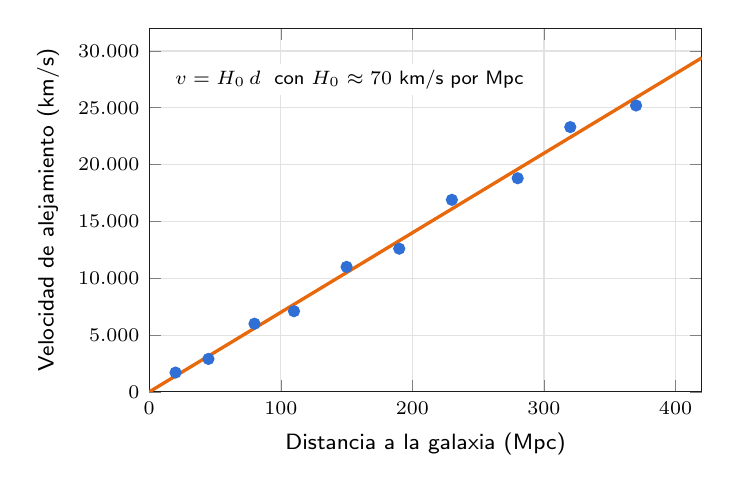
\begin{tikzpicture}[font=\footnotesize]
\begin{axis}[width=8.6cm,height=6.2cm,xmin=0,xmax=420,ymin=0,ymax=32000,
  xlabel={Distancia a la galaxia (Mpc)},ylabel={Velocidad de alejamiento (km/s)},
  scaled y ticks=false,ytick={0,5000,10000,15000,20000,25000,30000},
  yticklabel style={/pgf/number format/fixed},
  grid=major,grid style={gris!20},axis line style={tinta},tick label style={font=\scriptsize},label style={font=\footnotesize}]
\addplot[nar,very thick,domain=0:420] {70*x};
\addplot[only marks,mark=*,mark size=2pt,azul] coordinates {(20,1700)(45,2900)(80,6000)(110,7100)(150,11000)(190,12600)(230,16900)(280,18800)(320,23300)(370,25200)};
\node[anchor=west,font=\scriptsize,fill=white,inner sep=2pt] at (axis cs:15,27500) {$v = H_0\, d$ \ con $H_0 \approx 70$ km/s por Mpc};
\end{axis}
\end{tikzpicture}
\end{document}
